\chapter{Silicon Detectors for High Energy Physics}
\label{chap:silicon}

Pixel and strip detectors realised on high resistivity silicon substrates are nowadays the standard 
choice for high energy physics experiments. 
In this Chapter an introduction to silicon detectors will be given, focusing 
on those aspects that are relevant for the purpose of tracking and vertexing.
Excellent books on the subject exists, like~\cite{Lutz:411172,Sze1981,Wang1989}. Here 
some extracts from those will be reported, just to introduce the subject. 

 After reviewing the basics of the subject a discussion on radiation damage in silicon 
will follow in Section~\ref{sec:RadDam}.
\section{Semiconductor Basics}

The physics of semiconductor devices is naturally dependent on the physics of semiconductor 
themselves~\cite{Sze1981}. In this brief introduction only crystalline semiconductors will be treated 
and with a particular focus on silicon. Most commonly used semiconductors are crystals with 
diamond (Si and Ge) or zinc blende ({\it e.g.} GaAs) lattice type. In Figure~\ref{fig:diamondLattice} 
a schematic view of the diamond lattice is presented.


\begin{figure}[htbp]
   \centering
   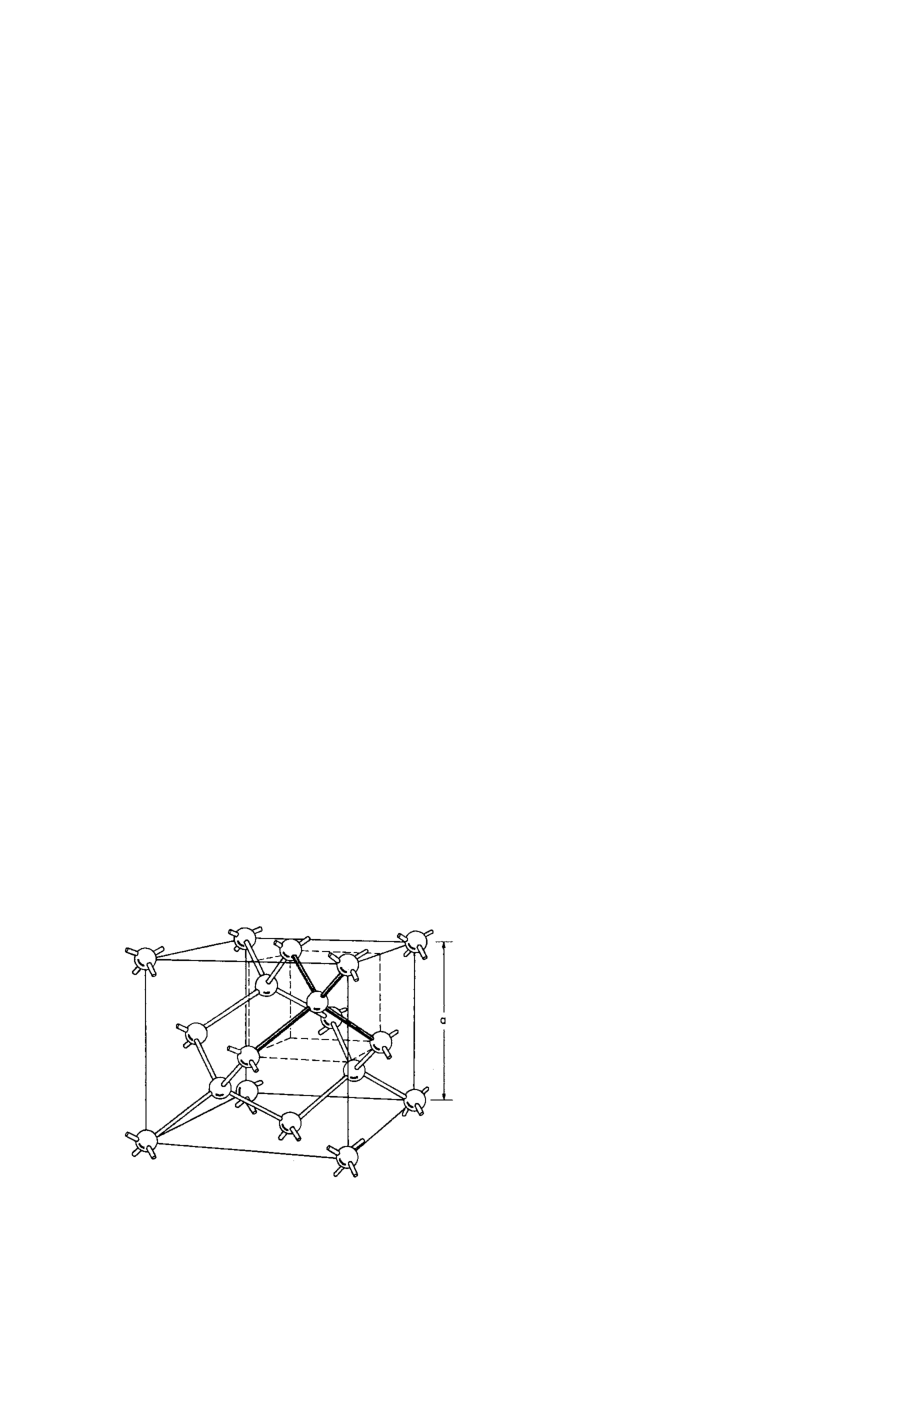
\includegraphics{diamondLattice.pdf} % requires the graphicx package
   \caption{\label{fig:diamondLattice}Diamond lattice. (After~\cite{Lutz:411172})}
\end{figure}

Due to the Pauli exclusion principle, electrons in crystals are organised in energy bands, 
each one containing many closely spaced levels. Figure~\ref{fig:EnergyLevels} helps in picturing 
the situation for diamond lattice: at very large distances each atom has the same two energy levels; 
the energy levels are $N$-fold degenerate ($N$ being the number of atoms), they indeed split 
into $N$ closely spaced levels when the atoms are brought close together. 
For $N\to\infty$, one speaks of energy bands, rather than levels, and these bands broaden, merge 
and split again with even closer spacing~\cite{Lutz:411172}.

\begin{figure}[htbp]
   \centering
   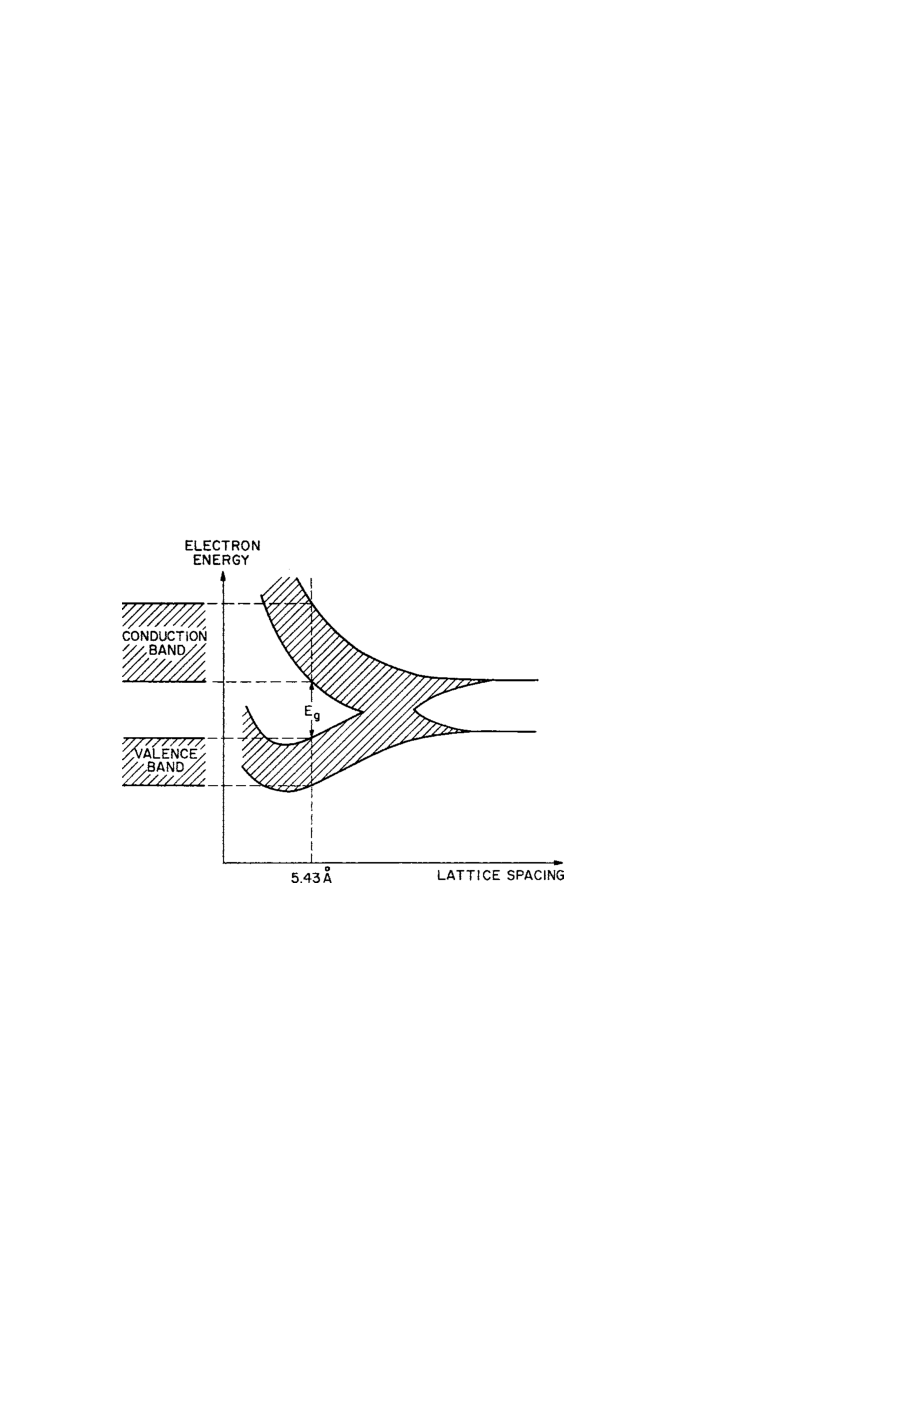
\includegraphics{EnergyLevels.pdf} % requires the graphicx package
   \caption{\label{fig:EnergyLevels}Energy levels of silicon atoms arranged in a diamond structure, as a function of lattice spacing. (After~\cite{Lutz:411172})}
\end{figure}

\section{Why Use Silicon}

Silicon detectors replaced the  gas based detectors in the tracking systems, since they offer a much
 better position information and an improved energy resolution. The reasons for this are to be found 
in the large density of silicon at room temperature, in the relatively low mean ionisation energy and 
in the possibility of use photolithography to realise charge collecting electrodes. 
These three characteristics allow to have large signals with a small active thickness and 
excellent spatial resolution. Some of the Silicon properties that are relevant for high energy 
physics applications are summarised in Table~\ref{tab:SiProperties}.

% Requires the booktabs if the memoir class is not being used
\begin{table}[htbp]
   \centering
   %\topcaption{Table captions are better up top} % requires the topcapt package
   \begin{tabular}{@{} lcr @{}} % Column formatting, @{} suppresses leading/trailing space
      \toprule
      \multicolumn{3}{c}{Silicon} \\
      \cmidrule(r){1-3} % Partial rule. (r) trims the line a little bit on the right; (l) & (lr) also possible
      Feature    & Value & Comments \\
      \midrule
      Density  $\rho$    & 2.33~g/cm${^3}$ & compact and thin detectors  \\
      Energy bandgap $E_g$ & 1.12~eV & non-cryogenic operation \\
      Ionisation energy $\epsilon$ & 3.6~eV & large signals\\
      Radiation length $X_0$      &  9.37~cm & thin detectors to minimize  \\
                                       &                 & multiple scattering \\
      Electron mobility  $\mu_e$     & $\sim$1350 cm$^2$V/s  & fast charge collection \\
      Saturation velocity $v_{sat}$ & $\sim$10$^{7}$ cm/s & fast charge collection \\
      \bottomrule
   \end{tabular}
   \caption{Summary of silicon properties relevant for high energy physics applications~\cite{Lutz:411172}.}
   \label{tab:SiProperties}
\end{table}

Other important characteristics that can explain the success of silicon are its large abundance, 
the possibility of changing its properties by doping, the existence of a natural oxide~\cite{Hartmann2012}.

\section{The p-n Junction}
\section{Silicon Trackers}
\section{Radiation Damage}
\label{sec:RadDam}
